% !TEX TS-program = pdflatex
% !TEX encoding = UTF-8 Unicode

% This is a simple template for a LaTeX document using the "article" class.
% See "book", "report", "letter" for other types of document.

\documentclass[12pt]{article} % use larger type; default would be 10pt

\usepackage[utf8]{inputenc} % set input encoding (not needed with XeLaTeX)

%%% Examples of Article customizations
% These packages are optional, depending whether you want the features they provide.
% See the LaTeX Companion or other references for full information.

%%% PAGE DIMENSIONS
\usepackage{geometry} % to change the page dimensions
\geometry{a4paper} % or letterpaper (US) or a5paper or....
\geometry{margin=1in} % for example, change the margins to 2 inches all round
% \geometry{landscape} % set up the page for landscape
%   read geometry.pdf for detailed page layout information

\usepackage{graphicx} % support the \includegraphics command and options

%%% PACKAGES
\usepackage{booktabs} % for much better looking tables
\usepackage{array} % for better arrays (eg matrices) in maths
\usepackage{paralist} % very flexible & customisable lists (eg. enumerate/itemize, etc.)
\usepackage{verbatim} % adds environment for commenting out blocks of text & for better verbatim
%\usepackage{subfig} % make it possible to include more than one captioned figure/table in a single float
\usepackage{pdfpages}
\usepackage{amsmath,mathtools,amsfonts}
\usepackage{bm}
\usepackage{blindtext}
\usepackage{fancyhdr}
\usepackage{float}
\usepackage{gensymb}
\usepackage{svg}
\usepackage{subcaption}

\graphicspath{ {./images/} }

%%% HEADERS & FOOTERS
\pagestyle{fancy}
\renewcommand{\headrulewidth}{1pt} % customise the layout...
\renewcommand{\footrulewidth}{1pt} % customise the layout...
%\renewcommand{\sectionmark}[1]{\markright{#1}}
%\renewcommand{\subsectionmark}[1]{\markright{#1}}
\fancyhf{}

% HEADER
\fancyhead[L]{ENEL321 Lab Report}
\fancyhead[C]{}
\fancyhead[R]{Jesse Sheehan}

% FOOTER
\fancyfoot[L]{\reflectbox{\includesvg[width=12pt]{rocket}}}
\fancyfoot[C]{\thepage}
\fancyfoot[R]{\includesvg[width=12pt]{rocket}}

%% TITLE
\title{\uppercase{
	Design, Implementation and Analysis of a Control System
}}
\date{\today}
\author{
	Jesse Patrick Sheehan\\
	\\
	{\small{ID: 53366509}}\\
	{\small{jps111@uclive.ac.nz}}\\
}

%\renewcommand{\sectionmark}[1]{\markright{\thesection\ #1}}

\begin{document}

\maketitle

\vfill

\begin{abstract}

% Motivation, what was done, summary of results (very brief)

\noindent The angle of a rotating boom on a test rig was required to be controlled.
P, PD, and PID control systems were created to meet the design specifications by responding to a step input.
The analysed results show that the none of the control systems met the design specifications but could meet them if certain changes were made.

\end{abstract}

\newpage

\section*{Methodology}

% Briefly introduce the problem, and experiment but don't derive the model.
A test rig (see figure \ref{fig:test-rig}), controlled by two brushless DC motors on its boom, is subjected to a 20\degree\ step input.

\begin{figure}[H]
	\centering
	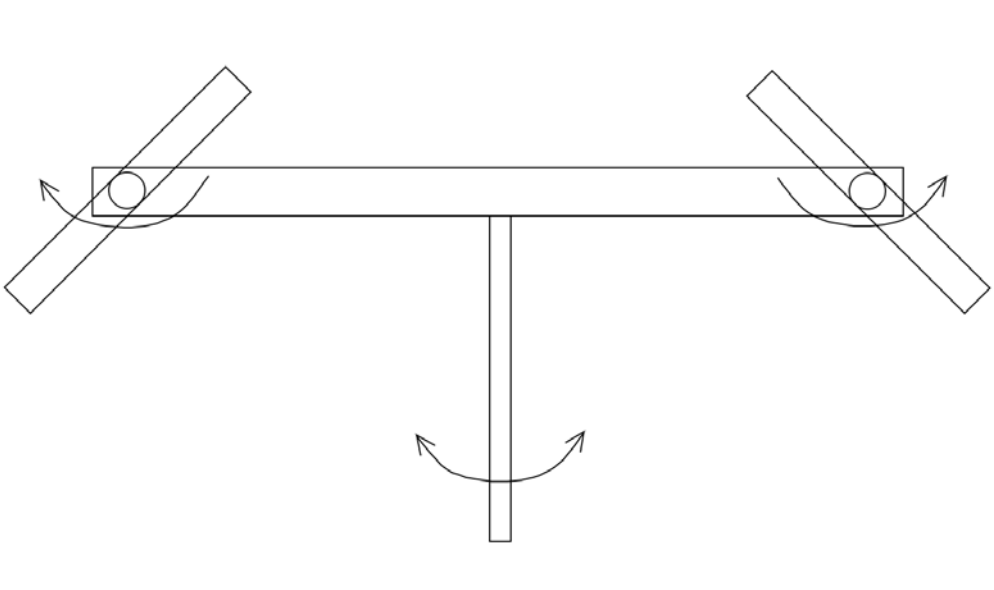
\includegraphics[scale=0.8]{test-rig}
	\caption{A front view of the test rig system (Hann, 2019).}
	\label{fig:test-rig}
\end{figure}

\noindent A feedback control system was designed and implemented to meet the following design specifications:
\begin{align*}
\xi &> 0.1 & M_p\% &< 15\%  \\[1em]
e_{ss} &< 1.5\degree & t_r &< 0.8 \textrm{s} \\[1em]
1 \leq K_p &\leq 2.5 & \frac{K_d}{K_p} &< 0.7
\end{align*}

% Explain how you designed your gains, and what values you used and why.
\noindent The predetermined gain values were found using an iterative approach. The transfer function (see equation\ \ref{eq:transfer-function}), with the suggested parameters $\alpha = 1.6$, $\beta = 2.9$, $\gamma = 1.3$ and $\tau = 0.34$, was used with MATLAB to predict how output would be affected by the gains and the step input.
\\ 

\begin{equation}
\label{eq:transfer-function}
\frac{X}{R} = \frac{\beta K_p s + \beta K_i}{s^3 + s^2 (\alpha + \beta K_d - \beta K_p \tau) + s(\gamma + \beta K_p - \beta K_i \tau) + \beta K_i}
\end{equation}
\\ 

\noindent Three sets of predetermined gain values were ultimately decided on:
\begin{align*}
\textrm{P controller} &: & K_p &= 1.20 & & & \\[1em]
\textrm{PD controller} &: & K_p &= 1.20 & K_d &= 1.20 & & \\[1em]
\textrm{PID controller} &: & K_p &= 1.20 & K_d &= 0.72 & K_i &= 0.84
\end{align*}

% Explain the different controllers used.
\noindent By using three different types of controller, we were able to analyse the differences between them and to better understand the relationship between the step input, the gains, and the output.
\\ 

\noindent The following expectations are visible in the MATLAB plot (figure\ \ref{fig:prelab}) below. The P controller would be expected to overshoot the target angle and then overshoot in the other direction, oscillating until it comes to a rest near the target angle. This would be an example of an underdamped system.
The PD controller would be expected to slowly converge upon the target angle with little or no overshoot (depending on the damping coefficient, $\xi$). A relatively large steady-state error ($e_{ss}$) would be expected. This would be an example of an overdamped system.
The PID controller is expected to overshoot but then quickly converge towards the target angle. This would be an example of a critically damped system.
\begin{figure}[H]
	\centering
	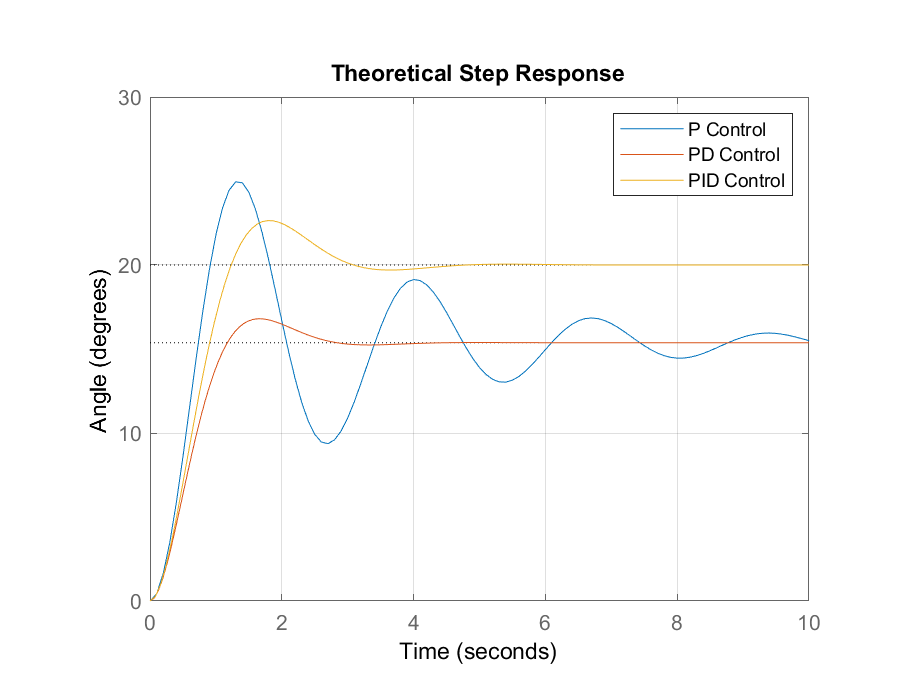
\includegraphics[scale=0.8]{prelab}
	\caption{The graph showing the predicted responses of each controller.}
	\label{fig:prelab}
\end{figure}

\newpage
\section*{Results}

% Present experimental results.
\noindent The following data (figures\ \ref{fig:pid-control},\ \ref{fig:pd-control},\ \ref{fig:pd-control}\ and table\ \ref{tab:results}) was captured during the lab:

\begin{figure}[H]
	\centering
	\begin{subfigure}[b]{0.9\textwidth}
		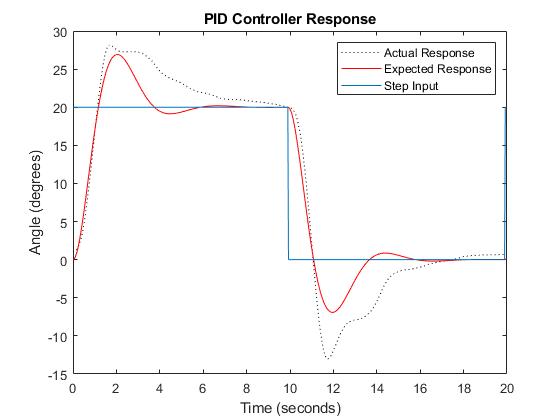
\includegraphics[width=\textwidth]{pid-control}
		\caption{PID controller response.}
		\label{fig:pid-control}
	\end{subfigure}
	\\[1em]
	\begin{subfigure}[b]{0.45\textwidth}
		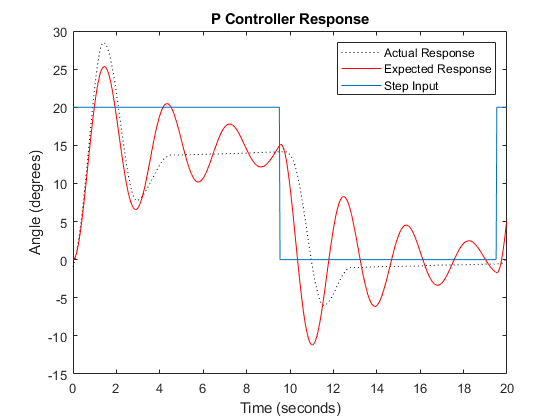
\includegraphics[width=\textwidth]{p-control}
		\caption{P controller response.}
		\label{fig:p-control}
	\end{subfigure}
	\begin{subfigure}[b]{0.45\textwidth}
		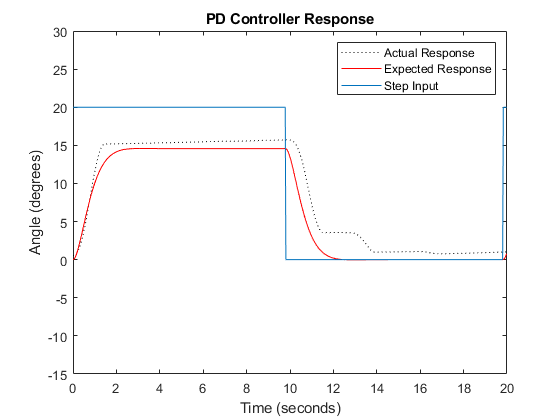
\includegraphics[width=\textwidth]{pd-control}
		\caption{PD controller response.}
		\label{fig:pd-control}
	\end{subfigure}
\end{figure}

\begin{table}[H]
\centering
\begin{tabular}{|l|l|l|l|l|l|l|}
	\hline
	\textbf{System} & $K_p$ & $K_d$ & $K_i$ & $M_p\ (\%)$ & $t_r\ \textrm{(s)}$ & $e_{ss}\ \textrm{(\degree)}$ \\
	
	\hline
	PID Control & 1.20 & 0.72 & 0.84 & 34.53 & 0.80 & 0.18 \\
	
	\hline
	P Control & 1.20 & 0.00 & 0.00 & 74.05 & 0.51 & 5.48 \\
	
	\hline
	PD Control & 1.20 & 1.20 & 0.00 & 0.21 & 1.30 & 5.44 \\
	
	\hline
\end{tabular}
\caption{The analysed results from the experiment.}
\label{tab:results}
\end{table}

\newpage
\section*{Discussion}

% Compare results with model, explain differences.
% Focus on the why rather than the what.

\noindent The experimental PID controller (figure\ \ref{fig:pid-control}) response was similar to its model. The main differences were the time taken to recover from an overshoot, which were longer than the model. However, the results show that the steady state was converging to within a degree of the target angle. This type of controller had the best steady-state error out of the three different control systems. This control system does not meet the design specifications due to the maximum overshoot being twice what it should.
\\

\noindent The P controller (figure\ \ref{fig:p-control}) was similar to the model, but with less oscillation involved. The oscillations subsided very quickly, whereas the model predicted that the oscillations would continue for a longer time period. The unexpected damping of the oscillations can be partially explained by the torque required to overcome static friction of the axle. Friction also existed from the USB cable that attached the microcontroller to the computer. This type of control system gave the quickest rise time, the largest maximum overshoot and a certain amount of steady-state error. This control system does not meet the design specifications due to the maximum overshoot and the steady-state error being too high.
\\ 

\noindent The PD controller (figure\ \ref{fig:pd-control}) increases the damping in the step response. The experimental results almost exactly match the model with the exception of the fall time being less (and therefore slower). A small anomoly exists in the data after the input falls from 20\degree\ to 0\degree. This may have been from having too much damping in the system. As expected, this control system had the smallest maximum overshoot. Like the P controller, the steady state error was almost 25\%. This control system does not satisfy the design specifications because of its steady-state error and rise times being too high.

\subsection*{Theoretical performance of $K_p$, $K_p$ and $K_d$}

\noindent Increasing the proportional gain reduces the rise time but increases the maximum overshoot. This may result in an unstable system if there not enough damping present. The proportional gain does not have a major impact on the steady-state error.
\\

\noindent Increasing the derivative gain causes the maximum overshoot to be less but increases the rise time. This is because it increases the overall damping in the system, allowing the response to slowly converge. Similar to $K_p$, $K_d$ does not have a great effect on the steady-state error. Increasing the derivative gain too much may make the system less responsive as it would have to overcome the high overall damping.
\\

\noindent Increasing the integral gain reduces the steady-state error and reduces the maximum overshoot. If there is not enough damping present in the system and the proportional gain is high enough the system may become unstable.

\newpage
\section*{Conclusion}

% Summarize what worked and what didn't, what could be improved as well as any limitations in the methods observed.
This report explored three different control system designs (P controller, PD controller and PID controller) intended to control a test rig with brushless DC motors. 
Of the three control system designs, none met the design specifications as intended due to several factors. The P controller increased the angle too fast causing a 74\% overshoot, the PD controller rise time increased too slowly and had a 25\% steady-state error, and the PID controller had a high maximum overshoot.
\\

\noindent A control system that has a fast rise time, small maximum overshoot and small steady-state error was not achieved but could be achieved after iterating on our suggested gain values.
Of the three candidate control systems, the PID controller was the closest in terms of meeting the design criteria.
To improve this, the integral gain could be reduced to reduce the maximum overshoot, or the derivative gain could be increased to provide more damping. This may lead to a system that can meet the design specifications.

\end{document}
